%%%%%%%%%%%%%%%%%%%%%%%%%%%%%%%%%%%%%%%%%%%%%%%%%%%%%%%%%%%%%%%%%
%  _____       ______   ____									%
% |_   _|     |  ____|/ ____|  Institute of Embedded Systems	%
%   | |  _ __ | |__  | (___    Wireless Group					%
%   | | | '_ \|  __|  \___ \   Zuercher Hochschule Winterthur	%
%  _| |_| | | | |____ ____) |  (University of Applied Sciences)	%
% |_____|_| |_|______|_____/   8401 Winterthur, Switzerland		%
%																%
%%%%%%%%%%%%%%%%%%%%%%%%%%%%%%%%%%%%%%%%%%%%%%%%%%%%%%%%%%%%%%%%%

\chapter{LaTeX Kurzanleitung}\label{chap.anleitung}
Dieses Kapitel führt mit Beispielcode in den LaTeX Code ein, und kann während der Erstellung des Dokuments gelöscht werden.\footnote{Verbesserungsvorschläge bitte an hegt@zhaw.ch senden}

Die nachfolgende Berichtstruktur wurde aus der Vorlage\footnote{Berichtstruktur Vorlage, Stand: August 2011} der \href{https://intra.zhaw.ch/departemente/school-of-engineering/studium-standort-winterthur/studierende/projektarbeit-bachelorarbeit.html}{PA/BA Termin-Webseite} vom ZHAW Intranet entnommen.

(): alle in Klammer aufgeführten Einträge sind situativ anzupassen



Das ist ein kleiner Text um zu zeigen, wie die Enter eingebracht werden.\\
Ich finde Latex schwierig.\\
Der Start ist echt eine Herausforderung. \\
Mensch ist das Komplex, echt was für Profis. % Hier brauchts ja kein Enter mehr, sonnst heisst es Overfull \hbox



\section{Visio Vektorgraphik einfügen}\label{visio}
(Graphik auswählen) Speichern unter -> PDF -> Optionen.. -> Auswahl\\
Mit Adobe Akrobat öffnen: Erweitert -> Druckproduktion -> Seiten beschneiden -> Weisse Ränder entfernen -> OK -> Ctrl-S

\begin{figure}[H]
	\centering
		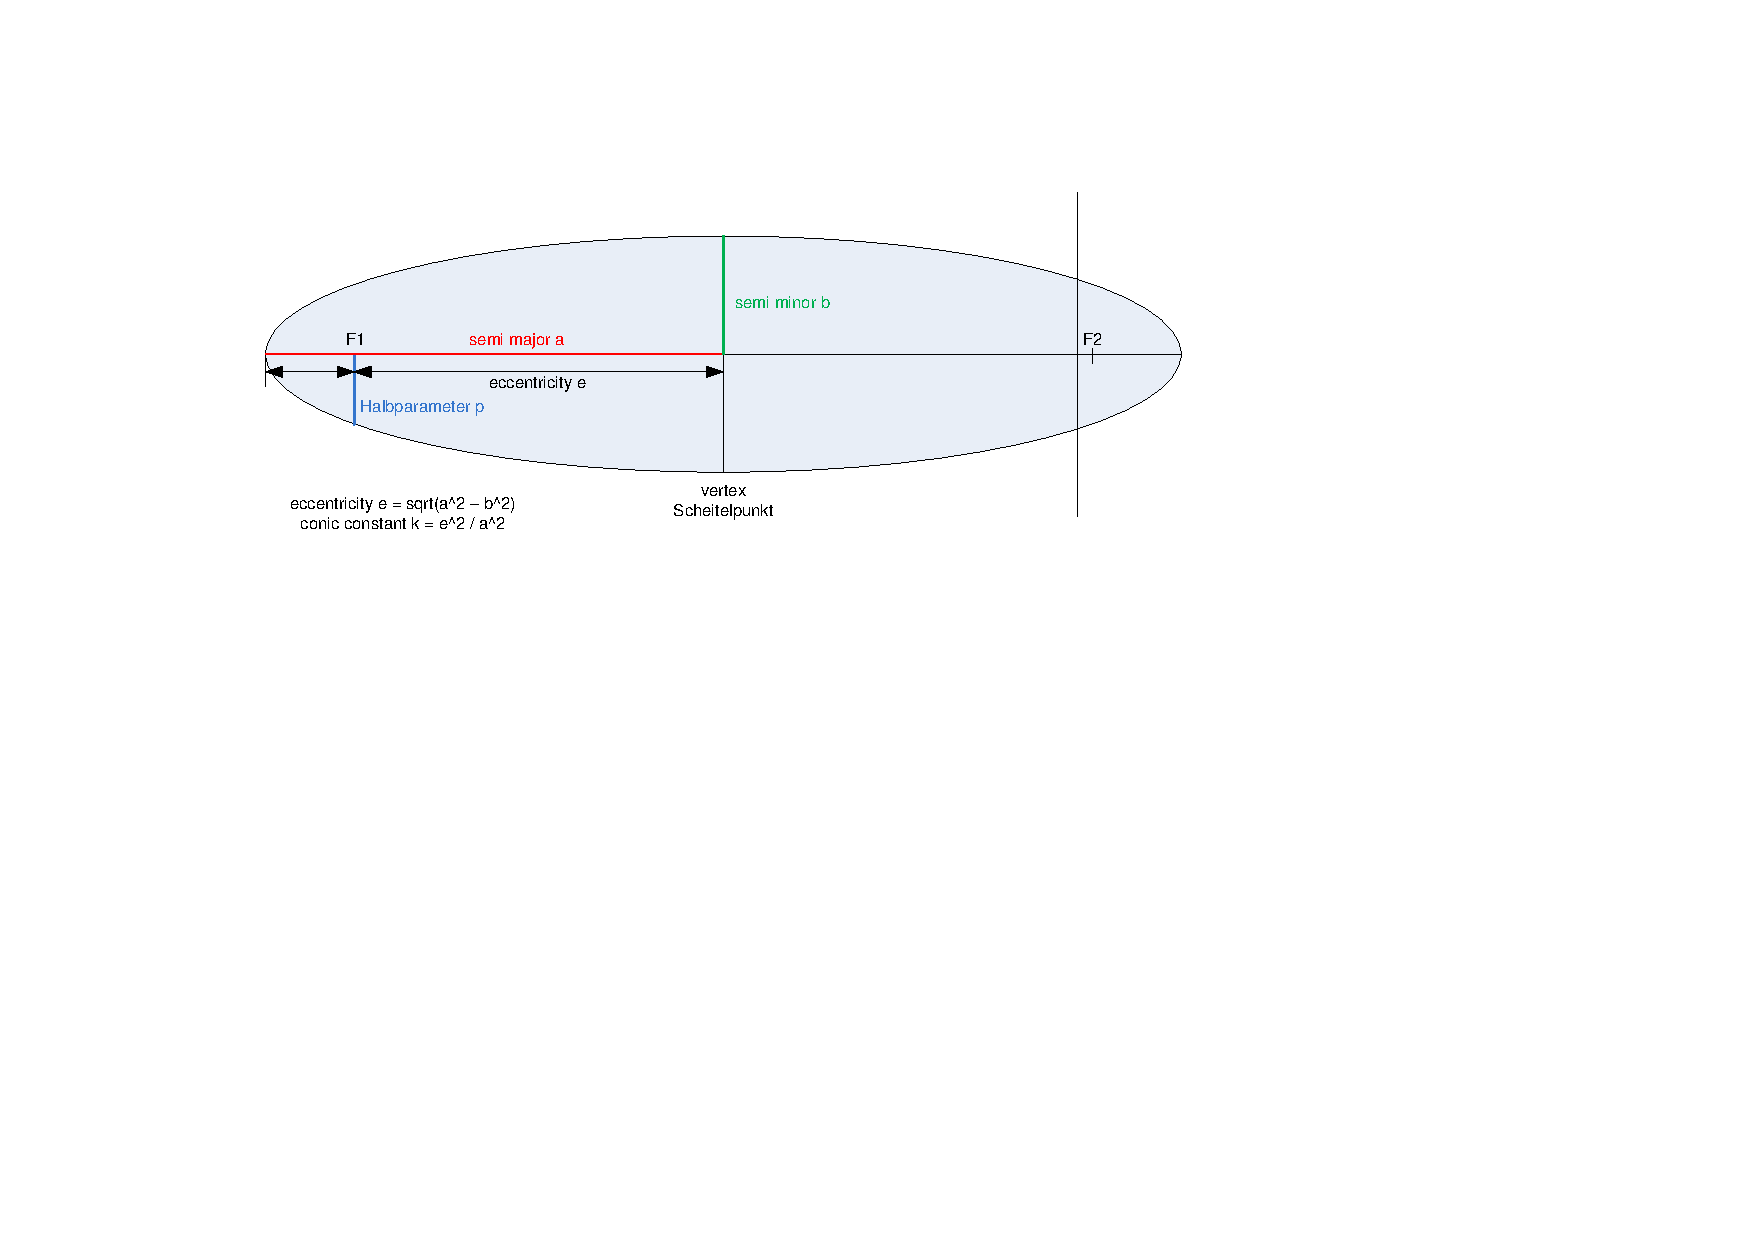
\includegraphics[width=0.8\textwidth]{images/visio/visio.pdf}
	\caption{Ideenskizze}
	\label{fig.Skizze}
\end{figure}

So kann die Abbildung~\ref{fig.Skizze} referenziert werden. Bei der PDF Erstellung ist darauf zu achten, dass LaTeX nur Versionen bis 1.4 voll unterstützt. 



\subsection{Graphiken in LaTeX zuschneiden}\label{zuschneiden}
Mit dem Befehl Clip kann eine Graphik auch in LaTeX zugeschnitten werden:

\begin{figure}[H]
	\centering
		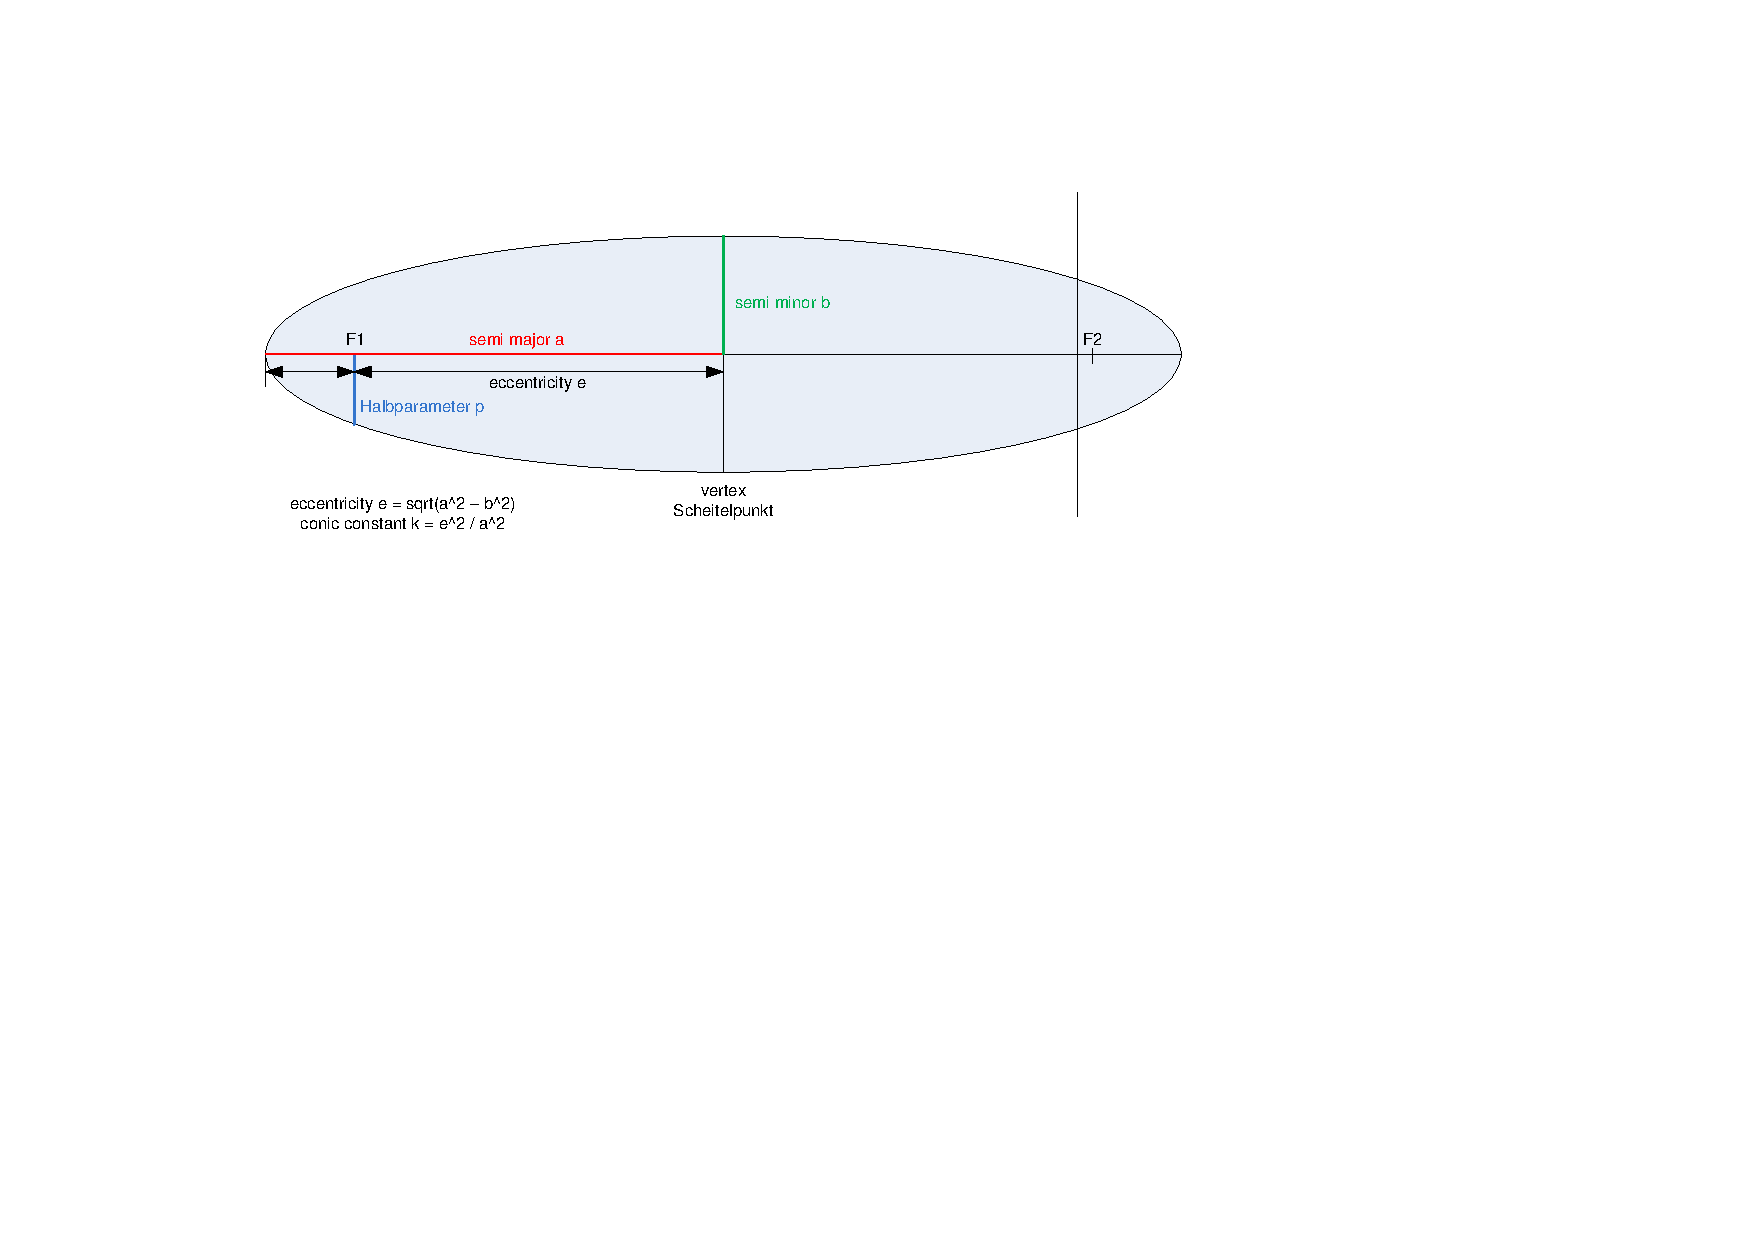
\includegraphics[width=0.9\textwidth, clip=true, trim = 80 10 0 10]{images/visio/visio.pdf}  % trim lm bm rm tm (left, bottom, right, top)
	\caption{clip=true, trim = 60 10 0 10}
	\label{fig.SkizzeZugeschnitten}
\end{figure}



\subsection{Mehrere Bilder nebeneinander}\label{nebeneinander}
Dank Minipages können mehrere Bilder auch nebeneinander sein:

%Zwei Bilder nebeneinander http://latex.mschroeder.net/
\begin{figure}[H]
  \centering
  \begin{minipage}[b]{0.45\textwidth}
    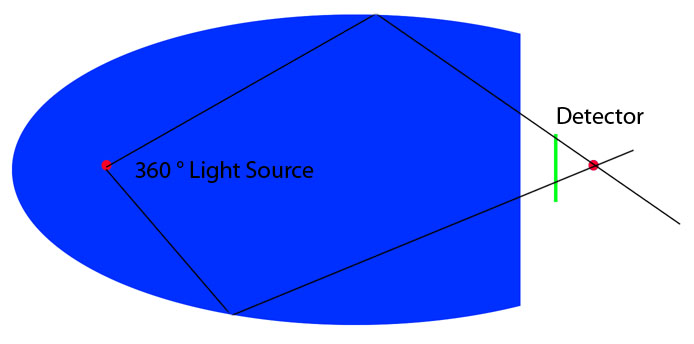
\includegraphics[scale=0.15]{images/photoshop/Skizze.jpg}
    \caption{Visir10b Detector}
    \label{Visir10bDetector} 
  \end{minipage} % Hier darf keine Leerzeile zwischen den beiden Minipages liegen!
  \begin{minipage}[b]{0.45\textwidth}
    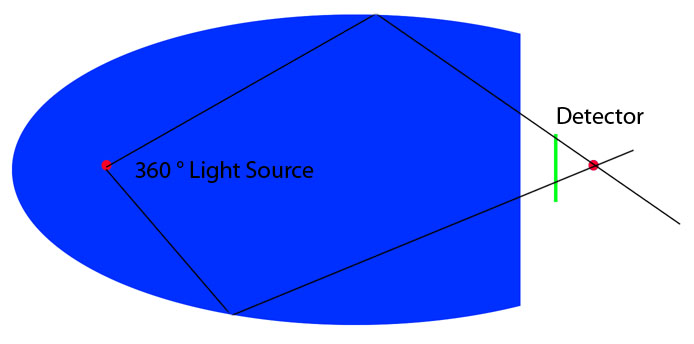
\includegraphics[scale=0.15]{images/photoshop/Skizze.jpg} 
    \caption{Visir10b Model}
    \label{Visir10bModel} 
  \end{minipage}
  \caption{Visir 10 mit optimiertem Reflektor}
  \label{fig.Visir10b}
\end{figure}


Literaturverweis: \citep{analog_devices_dac} \citep{microchip_spi}

\section{Tabellen aufbauen}\label{tabelle}
Kleine Tabelle:

\begin{table}[ht] \centering
	\begin{tabular}{|p{3cm}|p{.5cm}|p{.5cm}|p{.5cm}|p{.5cm}|p{.5cm}|p{.5cm}|p{.5cm}|p{.5cm}|p{.5cm}|p{.5cm}|} \hline
		\rowcolor{gray} Modul & M01 & M02 & M03 & M04 & M05 & M06 & M07 & M08 & M09 & M10 \\
		\hline
		FPGA\_DATEN & & & & & X & X & & X & X & \\
		\hline
		IRQ & X & X & X & & X & & & & X & X \\
		\hline
		Nachbar Core & & & & X & & X & & X & & \\
		\hline
	\end{tabular}
	\caption{Port Schwierigkeiten der Funkmodule}
	\label{tab:portprobleme}
 \end{table}	

Die nachfolgende longtable kann sich über mehrere Seiten erstrecken.

\begin{longtable}{|p{1.1cm}|p{4cm}|p{4cm}|p{4cm}|} 
					\hline
					\rowcolor{gray} Typ & Variante A & Variante B & Variante C
					\\ \hline
					& \textbf{Vorteile:} 
							\begin{itemize}
								\item[+] hohe Spannungen
							\end{itemize}							
							\textbf{Nachteile:}
							\begin{itemize}
								\item[-] Grosse Abmessung
							\end{itemize}
					& 	\textbf{Vorteile:} 
							\begin{itemize}
								\item[+] einfache Montage
							\end{itemize}							
							\textbf{Nachteile:}
							\begin{itemize}
								\item[-] max. 2A Eingangsstrom
							\end{itemize}
					&	\textbf{Vorteile:} 
							\begin{itemize}
								\item[+] hoher Strom
							\end{itemize}							
							\textbf{Nachteile:}
							\begin{itemize}
								\item[-] max. 12 V Eingangsspannung
							\end{itemize}\\ \hline
						Zeit & 2 h & 5 h & 3 h \\ \hline
						Preis	& 520 CHF/Stück & 800 CHF/Stück &	360 CHF/Stück\\ \hline
				\caption{Morphologischer Kasten für die Speisung}
				\label{tab:morphkasten}
			\end{longtable}	

Diese Art von Tabelle erstreckt sich immer auf der ganzen Seitenlänge:

\begin{tabularx}{\textwidth}{XXl}
  Salat & Schnecke & Igel\\
  Montag & Hier ist ein langes Wort & Dienstag
\end{tabularx}



\section{Code Listings aufbauen}\label{listing}

\begin{lstlisting}[
    language=C++,
    caption={Test Kommandozeilen Ausgabe},
    label={list.Testoutput}
]
/********************************************************/
/* Name        : M07Setup                               */
/* Description : EM9201 init for adress and pck         */
/* Input       : targetadr (DevAdr_M00 - DevAdr_M39)    */
/*               drate (Drate_M00 - Drate_M39)          */
/* Ouput       : -0x01 -> Setup OK                      */
/*               -0x5E -> Setup Error Channel write     */
/*               -0x6E -> Setup Error power write       */
/*               -0x7E -> Error in Device Address       */
/*               -0x8E -> Error in Peer Address         */
/********************************************************/
\end{lstlisting}

Formula $e = \sqrt{a{^2} - b^{2}}$


Diese Textstelle ist sehr interessant.\label{interessant}\\
Hier wird auf die Textstelle~\ref{interessant} verwiesen, die sich auf der Seite~\pageref{interessant} befindet.


% nogo:
% \ref{src:miktex} (\nameref{src:miktex})



\section{Citation nach IEEE}\label{citation}

Das ist ein \cite{robotvision} Verweis aufs Literaturverzeichnis. Ein anderes Beispiel ist das hier \cite{randompatterns}.





Das ist eine Aufzählung:
\begin{itemize} %
	\item Erste Zeile
	\item Zweite Zeile
	\item Dritte Zeile
\end{itemize}


\begin{enumerate}
\item erstens
\item zweitens
\end{enumerate}

%https://parma.zhaw.ch/svn/zhw_latex/
%gmanstyle nötig unter start od begin einbinden


Das ist eine verschachtelte Aufzählung:
\begin{description}
		\item [Register Performance] Alle Signale die das FPGA nicht verlassen, also von FF zu FF weitergeleitet werden. Daraus ergibt sich die maximale Taktfrequenz F\textsubscript{MAX}.

		\item [Externes Timing] FPGA Ein- und Ausgänge
		\begin{itemize}
			\item Ausgänge = Von FF's durch Logik zu Ausgängen (t\textsubscript{CO})
			\item Eingänge = Von Eingängen durch Logik zu FF's (t\textsubscript{SU}, t\textsubscript{H})
			\item Durchgänge = kombinatorische Pfade durch das FPGA (t\textsubscript{PD})
		\end{itemize}
\end{description}
